\documentclass[a4paper,10pt]{article}
\documentclass[a4paper,12pt]{report}
\usepackage[english]{babel}
\usepackage[left=2cm,right=2cm,top=2cm,bottom=2cm]{geometry}
%\usepackage{mathtools}
\usepackage{amsthm}     % for definitions and theorems
\usepackage[many]{tcolorbox}    % boxes around definitions and theorems
%\usepackage{amsmath}
%\usepackage{nccmath}
\usepackage{amssymb}    % \ltimes
\usepackage{etoolbox}   % for start of Chapter
%\usepackage{amsfonts}
\usepackage{physics}    % for all Physics related
\usepackage{dsfont}     % for the identity matrix symbol \1
%\usepackage{mathrsfs}

\usepackage{titling}
\usepackage{indentfirst}

\usepackage{bm}
\usepackage[dvipsnames]{xcolor}
\usepackage{cancel}

\usepackage{xurl}
\usepackage[colorlinks=true]{hyperref}

\usepackage{float}
\usepackage{graphicx}
\usepackage{subcaption}
%\usepackage{tikz}

\usepackage{ctable}     % tabelas
\renewcommand{\P}{\phantom{+}}  % empty space to indent things
\usepackage{multirow}
\usepackage{tabulary}

%%%%%%%%%%%%%%%%%%%%%%%%%%%%%%%%%%%%%%%%%%%%%%%%%%%

\newcommand{\eps}{\epsilon}
\newcommand{\vphi}{\varphi}
\newcommand{\cte}{\text{cte}}

\newcommand{\N}{{\mathbb{N}}}
\newcommand{\Z}{{\mathbb{Z}}}
%\newcommand{\Q}{{\mathbb{Q}}}
\newcommand{\C}{{\mathbb{C}}}
\renewcommand{\S}{{\hat{S}}}
%\renewcommand{\H}{\s{H}}

\renewcommand{\a}{{\vb{a}}}
\renewcommand{\b}{{\vb{b}}}
\renewcommand{\d}{{\dagger}}
\newcommand{\up}{{\uparrow}}
\newcommand{\down}{{\downarrow}}
\newcommand{\hc}{{\text{h.c.}}}

\newcommand{\ihat}{\bm{\hat{\imath}}}
\newcommand{\jhat}{\bm{\hat{\jmath}}}
\newcommand{\khat}{\bm{\hat{k}}}

\newcommand{\0}{{\vb{0}}}
\newcommand{\1}{\mathds{1}}
\newcommand{\E}{{\vb{E}}}
\newcommand{\B}{{\vb{B}}}
\renewcommand{\u}{{\vb{u}}}
\renewcommand{\v}{{\vb{v}}}
\renewcommand{\r}{{\vb{r}}}
\newcommand{\R}{{\vb{R}}}
\newcommand{\Q}{{\vb{Q}}}
\newcommand{\G}{{\vb{G}}}
\newcommand{\g}{{\vb{g}}}
\renewcommand{\k}{{\vb{k}}}
\newcommand{\K}{{\vb{K}}}
\newcommand{\p}{{\vb{p}}}
\newcommand{\q}{{\vb{q}}}
\newcommand{\F}{{\vb{F}}}
\renewcommand{\t}{{\vb{t}}}
\newcommand{\vtau}{{\bm{\tau}}}
\newcommand{\vdelta}{{\bm{\delta}}}

% COLORED SYMMETRY ELEMENTS
\newcommand{\Ct}{{\textcolor{Cyan}{C_3}}}
\newcommand{\Ctn}[1]{{\textcolor{Cyan}{C_3^{\textcolor{black}{#1}}}}}
\newcommand{\Cs}{{\textcolor{ForestGreen}{C_6}}}
\newcommand{\Csn}[1]{{\textcolor{ForestGreen}{C_6^{\textcolor{black}{#1}}}}}
\newcommand{\sd}{{\textcolor{RoyalBlue}{\sigma_d}}}
\newcommand{\sdn}[1]{{\textcolor{RoyalBlue}{\sigma_d^{\textcolor{black}{#1}}}}}
\newcommand{\sdp}{{\textcolor{RoyalBlue}{\sigma_d'}}}
\newcommand{\sdpp}{{\textcolor{RoyalBlue}{\sigma_d''}}}
\newcommand{\sv}{{\textcolor{Orange}{\sigma_v}}}
\newcommand{\svn}[1]{{\textcolor{Orange}{\sigma_v^{\textcolor{black}{#1}}}}}
\newcommand{\svp}{{\textcolor{Orange}{\sigma_v'}}}
\newcommand{\svpp}{{\textcolor{Orange}{\sigma_v''}}}

\newcommand{\s}{\sigma}
%\newcommand{\prodint}[2]{\left\langle #1 , #2 \right\rangle}
\newcommand{\cc}[1]{\overline{#1}}
\newcommand{\Eval}[3]{\eval{\left( #1 \right)}_{#2}^{#3}}
\newcommand{\sg}[2]{\{ #1 \mid #2 \}}

\newcommand{\unit}[1]{\; \mathrm{#1}}

\newcommand{\n}{\medskip}
\newcommand{\e}{\quad \mathrm{and} \quad}
\newcommand{\ou}{\quad \mathrm{or} \quad}
\newcommand{\virg}{\, , \;}
\newcommand{\ptodo}{\forall \,}
\renewcommand{\implies}{\; \Rightarrow \;}
%\newcommand{\eqname}[1]{\tag*{#1}} % Tag equation with name

\setlength{\droptitle}{-7em}

\makeatletter
\patchcmd{\chapter}{\if@openright\cleardoublepage\else\clearpage\fi}{}{}{}  % start 'Chapter' at the same page. needs package etoolbox
\makeatother

%% Theorems, definitions, proofs
\theoremstyle{definition}

\newtheorem{definition}{Definition}[section]
\tcolorboxenvironment{definition}{
  colback=blue!5!white,
  boxrule=0pt,
  boxsep=1pt,
  left=2pt,right=2pt,top=2pt,bottom=2pt,
  oversize=2pt,
  sharp corners,
  before skip=\topsep,
  after skip=\topsep,
}

\newtheorem{theorem}{Theorem}[section]
\tcolorboxenvironment{theorem}{
  colback=blue!5!white,
  boxrule=0pt,
  boxsep=1pt,
  left=2pt,right=2pt,top=2pt,bottom=2pt,
  oversize=2pt,
  sharp corners,
  before skip=\topsep,
  after skip=\topsep,
}


%\documentclass[../main.tex]{subfiles}
%\graphicspath{{\subfix{../fig/}}}

\begin{document}

Throughout our work, $\hbar = 1$.

\n

Graphene is an allotrope of graphite and consists of a hexagonal lattice of carbon atoms linked in $sp^2$ hybridization with distance $a$, where $3$ electrons from carbon form $\s$ bonds and the last electron is located on a $\pi$ orbital and is the only one that matters for the electronic properties of the material.

\n

Our convention is zig-zag in horizontal direction and arm-chair in vertical direction.

\begin{figure}[H]
\centering
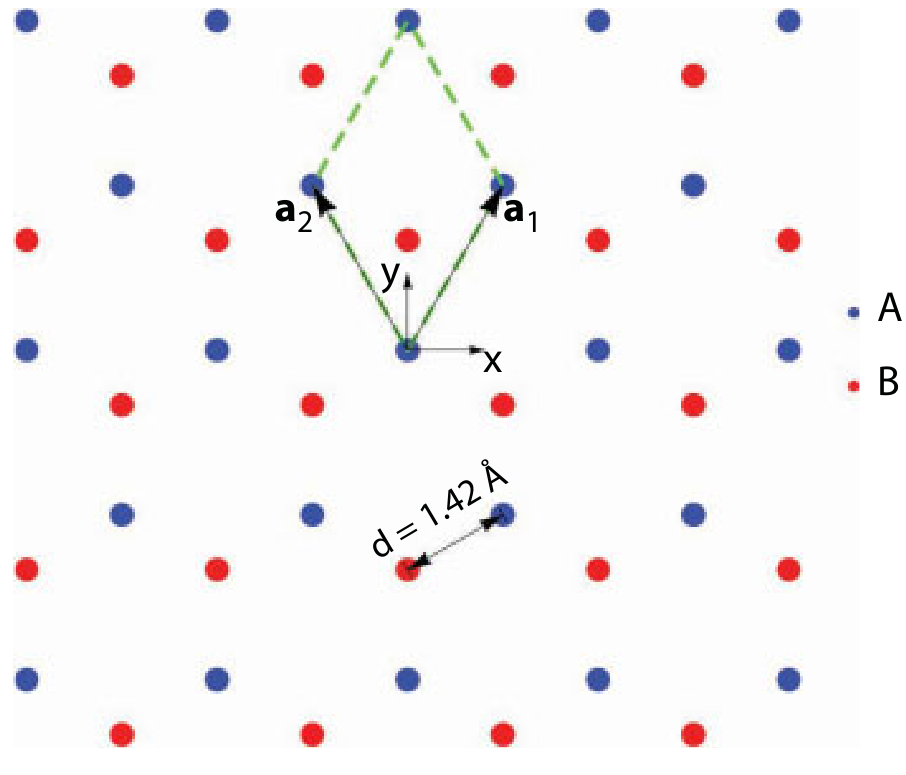
\includegraphics[width=0.4\linewidth]{fig/graphene-lattice_vectors2.png}
\label{fig:graphene-lattice_vectors}
\caption{Graphene lattice vectors. Taken from \cite{handbook2019}}
\end{figure}

The lattice vectors are $\vb{a}_1 = a \qty(\frac{1}{2}, \frac{\sqrt{3}}{2})$, $\vb{a}_2 = a \qty(-\frac{1}{2}, \frac{\sqrt{3}}{2})$. The unit cell area is
$$
A = \abs{\a_1 \times \a_2} = \frac{\sqrt{3}}{2} a^2.
$$

The Brillouin zone is
\begin{figure}[H]
\centering
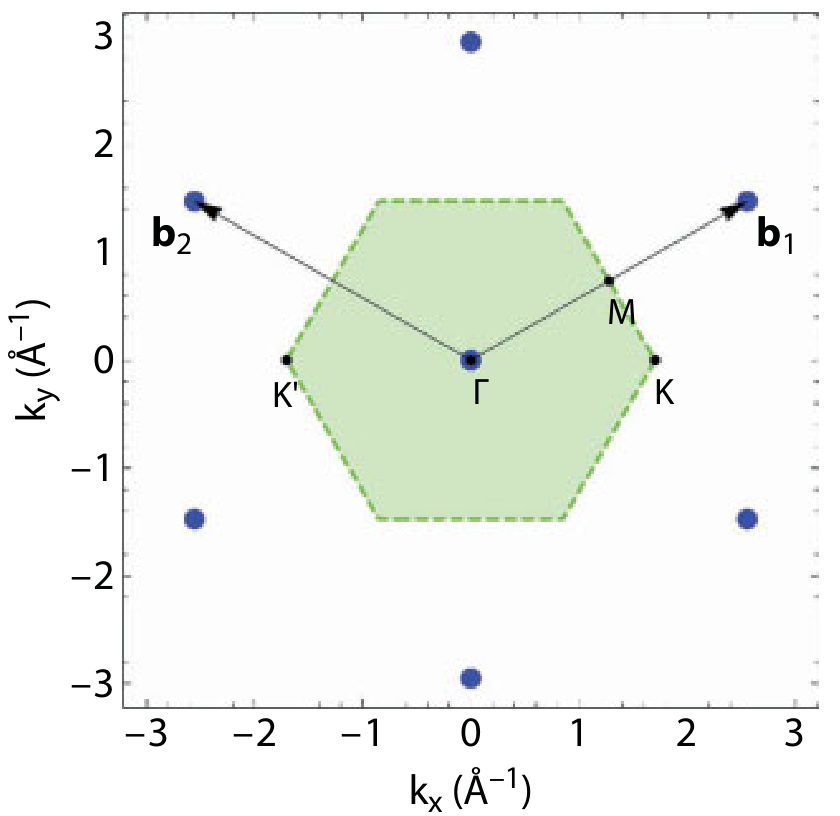
\includegraphics[width=0.3\linewidth]{fig/brillouin-zone-monolayer.png}
\caption{}
\label{fig:brillouin-zone-monolayer}
\end{figure}

where ($\a_3 = \vu{z}$)
$$
\b_1 = \frac{2\pi}{A} \a_2 \times \a_3 = \frac{4\pi}{\sqrt{3} a } \qty(\frac{\sqrt{3}}{2}, \frac{1}{2}),
$$
$$
\b_2 = \frac{2\pi}{A} \a_3 \times \a_1 = \frac{4\pi}{\sqrt{3} a } \qty(-\frac{\sqrt{3}}{2}, \frac{1}{2}).
$$

The Dirac points are defined as
$$
\K = \frac{4\pi}{3a} (1, 0) , \quad \K' = -\K.
$$



We write a tight-binding hamiltonian with only nearest-neighbor hopping
$$
H = -t \sum_{\R} c^\d_B(\R) \qty(c_A(\R) + c_A(\R-\a_1) + c_A(\R-\a_2)) + \hc,
$$
where the $\R$ sum runs through all the associated Bravais triangular lattice. Applying the Fourier transforms
$$
c_{\alpha}^\d(\R) = \frac{1}{\sqrt{N}} \sum_{\k \in \text{BZ}} e^{-i \k \vdot \r_i} c_A^\d(\k),
$$
we get
$$
H = \sum_{\k}
\begin{pmatrix}
c_A^\d(\k) & c_B^\d(\k)
\end{pmatrix}
\begin{pmatrix}
0 & -t f(\k) \\
-t f^*(\k) & 0
\end{pmatrix}
\begin{pmatrix}
c_A^\d(\k) \\ c_B^\d(\k)
\end{pmatrix},
$$
with
$$
f(\k) = \sum_{\nu} e^{i \k \vdot \bm{\delta}_\nu} =
e^{idk_y} + 2 e^{-\frac{idk_y}{2}} \cos(\frac{\sqrt{3}}{2} dk_x),
$$
where $\bm{\delta}_1 = (\a_1 + \a_2)/3 = d (0, 1)$, $\bm{\delta}_2 = (-2\a_1 + \a_2)/3 = d(-\frac{\sqrt{3}}{2}, -\frac{1}{2})$, $\bm{\delta}_3 = (\a_1 - 2\a_2)/3 = d (\frac{\sqrt{3}}{2}, -\frac{1}{2})$ are the vectors that connect to the three nearest neighboring sites, and $d = a/\sqrt{3}$.

The eigenenergies are $E_\pm(\k) = \pm t \abs{f(\k)}$.

\n

If we define $\K = \frac{4\pi}{3a} (1, 0)$, notice that the points $\K$ and $\K'=-\K$ are roots of $f$, i.e., $f(\pm\K) = 0$.


These are the so-called Dirac points, around which the dispersion relation are approximately linear $E(\K + \q) = v_F \abs{\q} + O\qty[\qty(\frac{\abs{\q}}{\abs{\K}})^2]$.


%%-----
%% Referências bibliográficas
%%-----
\addcontentsline{toc}{chapter}{\bibname}
%\bibliographystyle{abntex2-num}
\bibliography{citations}
\bibliographystyle{ieeetr}


\end{document}
